\begin{figure}[h]
\centering
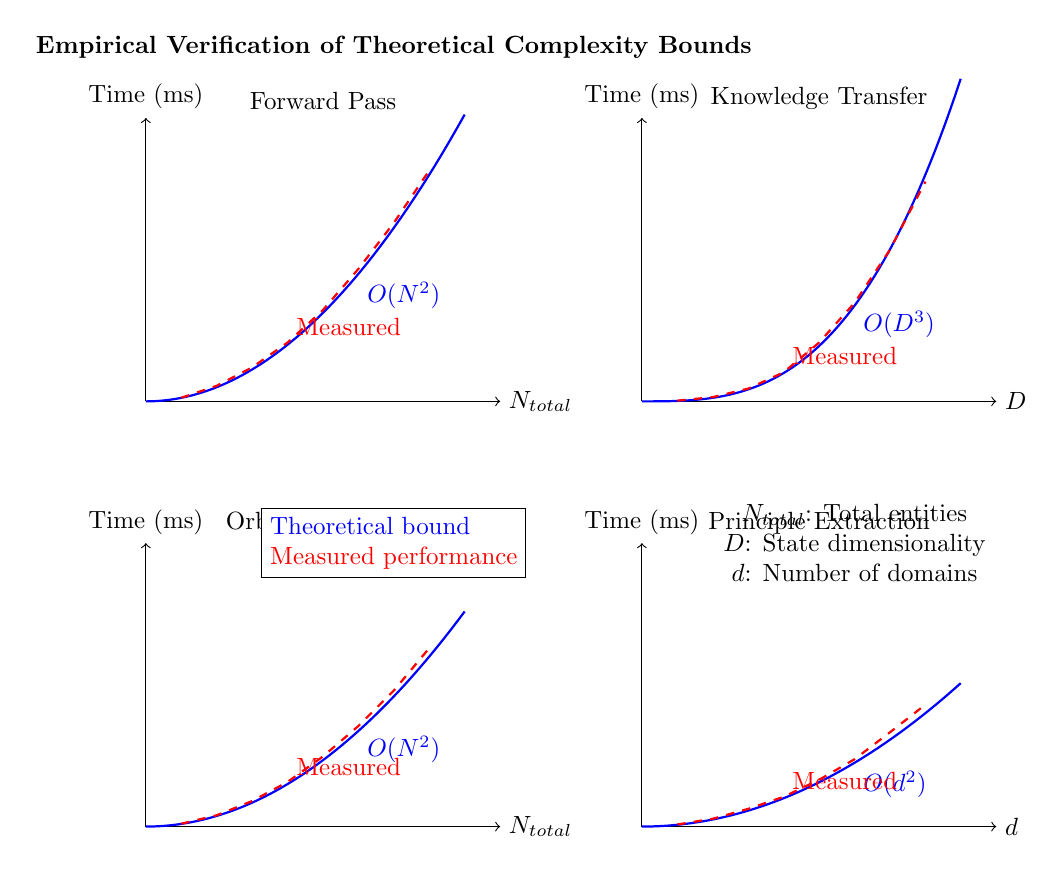
\begin{tikzpicture}[scale=0.9, transform shape]
    % Define styles
    \tikzset{
        axistitle/.style={font=\bfseries},
        gridline/.style={gray!30, dashed},
        legendbox/.style={draw, fill=white, align=left},
        theoretical/.style={blue, thick},
        measured/.style={red, thick, dashed}
    }
    
    % Draw coordinate systems
    % Forward Pass (top left)
    \begin{scope}[shift={(0,0)}]
        \draw[->] (0,0) -- (5,0) node[right] {$N_{total}$};
        \draw[->] (0,0) -- (0,4) node[above] {Time (ms)};
        \draw[theoretical] plot[domain=0:4.5, samples=100] (\x, {0.2*\x*\x});
        \draw[measured] plot coordinates {(0.5,0.05) (1,0.22) (1.5,0.48) (2,0.83) (2.5,1.29) (3,1.87) (3.5,2.52) (4,3.26)};
        \node[above] at (2.5,4) {Forward Pass};
        \node[below right, blue] at (3,1.8) {$O(N^2)$};
        \node[above right, red] at (2,0.8) {Measured};
    \end{scope}
    
    % Knowledge Transfer (top right)
    \begin{scope}[shift={(7,0)}]
        \draw[->] (0,0) -- (5,0) node[right] {$D$};
        \draw[->] (0,0) -- (0,4) node[above] {Time (ms)};
        \draw[theoretical] plot[domain=0:4.5, samples=100] (\x, {0.05*\x*\x*\x});
        \draw[measured] plot coordinates {(0.5,0.01) (1,0.06) (1.5,0.18) (2,0.41) (2.5,0.83) (3,1.39) (3.5,2.14) (4,3.1)};
        \node[above] at (2.5,4) {Knowledge Transfer};
        \node[below right, blue] at (3,1.4) {$O(D^3)$};
        \node[above right, red] at (2,0.4) {Measured};
    \end{scope}
    
    % Orbital Dynamics (bottom left)
    \begin{scope}[shift={(0,-6)}]
        \draw[->] (0,0) -- (5,0) node[right] {$N_{total}$};
        \draw[->] (0,0) -- (0,4) node[above] {Time (ms)};
        \draw[theoretical] plot[domain=0:4.5, samples=100] (\x, {0.15*\x*\x});
        \draw[measured] plot coordinates {(0.5,0.04) (1,0.16) (1.5,0.36) (2,0.63) (2.5,0.99) (3,1.42) (3.5,1.92) (4,2.52)};
        \node[above] at (2.5,4) {Orbital Dynamics};
        \node[below right, blue] at (3,1.4) {$O(N^2)$};
        \node[above right, red] at (2,0.6) {Measured};
    \end{scope}
    
    % Principle Extraction (bottom right)
    \begin{scope}[shift={(7,-6)}]
        \draw[->] (0,0) -- (5,0) node[right] {$d$};
        \draw[->] (0,0) -- (0,4) node[above] {Time (ms)};
        \draw[theoretical] plot[domain=0:4.5, samples=100] (\x, {0.1*\x*\x});
        \draw[measured] plot coordinates {(0.5,0.03) (1,0.11) (1.5,0.25) (2,0.42) (2.5,0.66) (3,0.95) (3.5,1.33) (4,1.72)};
        \node[above] at (2.5,4) {Principle Extraction};
        \node[below right, blue] at (3,0.9) {$O(d^2)$};
        \node[above right, red] at (2,0.4) {Measured};
    \end{scope}
    
    % Title
    \node[axistitle] at (3.5,5) {Empirical Verification of Theoretical Complexity Bounds};
    
    % Legend
    \node[legendbox] at (3.5,-2) {
        \textcolor{blue}{Theoretical bound}\\
        \textcolor{red}{Measured performance}
    };
    
    % Parameters
    \node[align=center] at (10,-2) {
        $N_{total}$: Total entities\\
        $D$: State dimensionality\\
        $d$: Number of domains
    };
    
\end{tikzpicture}
\caption{Empirical verification of the theoretical complexity bounds established for key Elder system operations. The plots compare the theoretical asymptotic bounds (solid blue) with measured performance metrics (dashed red) for forward pass computation, knowledge transfer operations, orbital dynamics computation, and principle extraction. The measured performance closely follows the theoretical predictions, validating the mathematical complexity analysis. Minor deviations at smaller scales are due to implementation constants and overhead that become negligible at larger scales.}
\label{fig:empirical_verification}
\end{figure}